% BÀI TOÁN HÌNH HỌC - BAI_HINH_21 (TRÍCH ĐỀ 21)
\begin{ex}
Cho $\triangle ABC$ có ba góc nhọn nội tiếp đường tròn (O) và $AB < AC$. Kẻ đường cao AD của tam giác ABC và đường kính AE của đường tròn tâm (O). Gọi F là chân đường vuông góc kẻ từ B xuống đường kính AE.
	\begin{enumerate}
		\item[a)] Chứng minh: bốn điểm A; B; D; F cùng thuộc một đường tròn.
		\item[b)] Chứng minh: $AB \cdot AC = AD \cdot AE$ và DF vuông góc với AC.
	\end{enumerate}
\loigiai{
{
	\begin{center}
		
		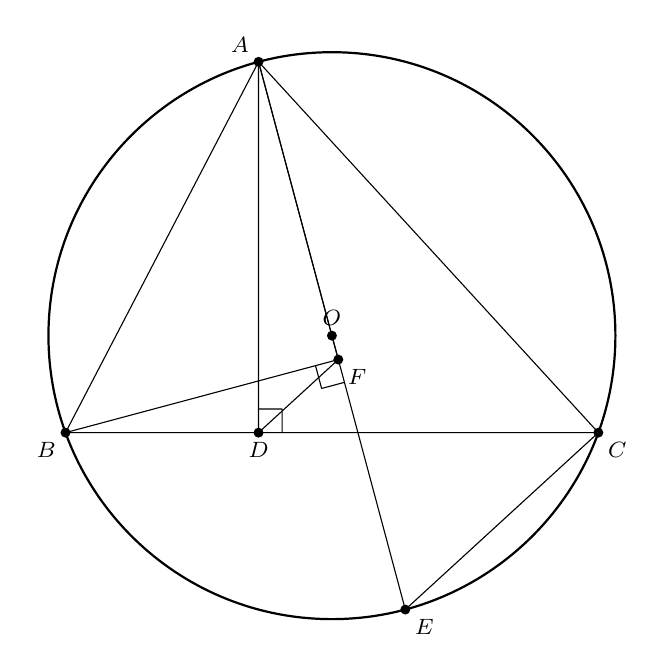
\begin{tikzpicture}[line join = round, line cap=round,>=stealth,font=\footnotesize,scale=1.2]
			\usetikzlibrary{calc,angles,quotes} % quotes for potential future use with angle labels
			% Def
			\def\r{3}
			
			% Coordinates
			\coordinate (O) at (0,0);
			\coordinate (B) at (-160:\r); % Điểm B
			\coordinate (C) at (-20:\r);  % Điểm C
			\coordinate (A) at (105:\r);  % Điểm A
			
			% D là hình chiếu của A lên BC
			\coordinate (D) at ($ (B)!(A)!(C) $);
			
			% E sao cho O là trung điểm của AE
			% E là điểm đối xứng của A qua O
			\coordinate (E) at ($ 2*(O) - (A) $); 
			% Hoặc \coordinate (E) at (105+180:\r);
			
			% F là hình chiếu của B lên AE
			\coordinate (F) at ($ (A)!(B)!(E) $);
			
			% Draw
			% Vẽ đường tròn (O,r)
			\draw[thick] (O) circle (\r);
			
			% Vẽ các đường A-B-C-A
			\draw (A) -- (B) -- (C) -- cycle;
			
			% Vẽ A-D
			\draw (A) -- (D);
			
			% Vẽ D-F
			\draw (D) -- (F);
			
			% Vẽ F-B
			\draw (F) -- (B);
			
			% Vẽ F-A (đoạn này là một phần của AE)
			\draw (F) -- (A); % Thực ra đã được bao gồm nếu vẽ AE, nhưng để rõ ràng
			
			% Vẽ A-E
			\draw (A) -- (E);
			
			% Vẽ E-C
			\draw (E) -- (C);
			
			% Fill points
			\fill (O) circle (1.5pt);
			\fill (A) circle (1.5pt);
			\fill (B) circle (1.5pt);
			\fill (C) circle (1.5pt);
			\fill (D) circle (1.5pt);
			\fill (E) circle (1.5pt);
			\fill (F) circle (1.5pt);
			
			% Node points (old style)
			\node[above] at (O) {$O$};
			\node[above left] at (A) {$A$};       % A ở góc phần tư II
			\node[below left] at (B) {$B$};       % B ở góc phần tư III
			\node[below right] at (C) {$C$};      % C ở góc phần tư IV
			\node[below] at (D) {$D$};            % D trên BC
			\node[below right] at (E) {$E$};      % E ở góc phần tư IV (đối xứng A qua O)
			\node[below right] at (F) {$F$}; % F trên AE, vị trí tương đối
			
			% Ký hiệu góc vuông (old style)
			% AD vuông góc BC
			\pic[draw, angle radius=3mm]{right angle = A--D--C}; % Giả sử D nằm giữa B và C, hoặc gần C
			% BF vuông góc AE
			\pic[draw, angle radius=3mm]{right angle = B--F--E}; % Giả sử F nằm giữa A và E
			
		\end{tikzpicture}
		
	
	\end{center}
}
\end{ex}
